% \documentclass{article}
% \usepackage{graphicx} % Required for inserting images

% \title{COL774 A3 Writeup}
% \author{Aman Hassan}
% \date{November 2023}

% \begin{document}

% \maketitle

% \section{Introduction}

% \end{document}

\documentclass[12pt]{article}
\usepackage[a4paper,margin=0.75in]{geometry}
\usepackage[utf8]{inputenc}
\usepackage[OT1]{fontenc}
\usepackage[table,usenames,dvipsnames]{xcolor}
\usepackage{array}
\usepackage{varwidth}
\usepackage{tabularx}
\usepackage{amsmath}
\usepackage{hyperref}
\usepackage{enumitem}
\usepackage{graphicx}
\usepackage{tcolorbox}
\renewcommand*\familydefault{\sfdefault}

\newtcolorbox{mybox}[3][]
{
  colframe = #2!25,
  colback  = #2!10,
  coltitle = #2!20!black,  
  title    = {#3},
  #1,
}

\hypersetup{
    colorlinks=true,
    linkcolor=blue,
    filecolor=magenta,      
    urlcolor=cyan,
    pdftitle={Overleaf Example},
    pdfpagemode=FullScreen,
}

\title{\textbf{COL774 Assignment 3}}
\author{Brian Sajeev Kattikat \\ \texttt{2021CS50609}}
\date{November 2023}

\begin{document}

\maketitle

\section{Decision Tree}

\begin{enumerate}[label=(\alph*)]

    \item Here we constructed the Decision Tree for varying depths where features to split are determined using highest mutual information metric
          \begin{enumerate}[label=\roman*.]
              \item
                    \begin{itemize}
                        \item Only Win:
                              \begin{itemize}
                                  \item Accuracy for in prediction type of only win on training set is 50.3380
                                  \item Accuracy for in prediction type of only win on test set is 49.6380
                              \end{itemize}
                        \item Only Loss
                              \begin{itemize}
                                  \item Accuracy for in prediction type of only loss on training set is 49.6614
                                  \item Accuracy for in prediction type of only loss on test set is 50.3619
                              \end{itemize}
                        \item DT with varying depths on training set:
                              \begin{itemize}
                                  \item Accuracy for depth 5 on training set is 88.55
                                  \item Accuracy for depth 10 on training set is 99.94
                                  \item Accuracy for depth 15 on training set is 100
                                  \item Accuracy for depth 20 on training set is 100
                                  \item Accuracy for depth 25 on training set is 100
                                  \item Accuracy for depth 30 on training set is 100
                              \end{itemize}
                        \item DT with varying depths on test set:
                              \begin{itemize}
                                  \item Accuracy for depth 5 on test set is 57.60
                                  \item Accuracy for depth 10 on test set is 60.19
                                  \item Accuracy for depth 15 on test set is 60.19
                                  \item Accuracy for depth 20 on test set is 60.19
                                  \item Accuracy for depth 25 on test set is 60.19
                              \end{itemize}
                    \end{itemize}
                    From the data obtained we find that single type prediction(only win, only loss) performs worse compared to Decision Tree classification (DT is almost 2x better in training prediction). As we expect the training accuracy is much better than test accuracy. We also find that the accuracy is almost the same after depth 10-15 ( This can be attributed to the aggressive terminating conditions applied on grow\_tree / fit function )
              \item The following Accuracy vs depth graph was obtained
          \end{enumerate}
          \begin{center}
              \begin{tabular}{c}
                  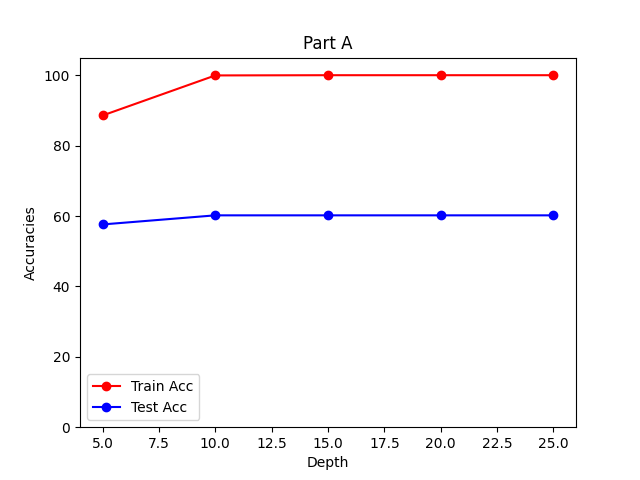
\includegraphics[width=0.9\textwidth]{./images/q1_part_a.png}
              \end{tabular}
          \end{center}

    \item Using one-hot encoding we obtain the following results

          \begin{enumerate}[label=\roman*.]
              \item
                    \begin{itemize}
                        \item Only Win:
                              \begin{itemize}
                                  \item Accuracy for in prediction type of only win on training set is 50.3386
                                  \item Accuracy for in prediction type of only win on test set is 49.6381
                              \end{itemize}
                        \item Only Loss
                              \begin{itemize}
                                  \item Accuracy for in prediction type of only loss on training set is 49.6614
                                  \item Accuracy for in prediction type of only loss on test set is 50.3619
                              \end{itemize}
                        \item DT with varying depths on training set:
                              \begin{itemize}
                                  \item Accuracy for depth 15 on training set is 70.59
                                  \item Accuracy for depth 25 on training set is 84.96
                                  \item Accuracy for depth 35 on training set is 92.60
                                  \item Accuracy for depth 45 on training set is 99.18
                              \end{itemize}
                        \item DT with varying depths on test set:
                              \begin{itemize}
                                  \item Accuracy for depth 15 on test set is 55.84
                                  \item Accuracy for depth 25 on test set is 61.74
                                  \item Accuracy for depth 35 on test set is 61.53
                                  \item Accuracy for depth 45 on test set is 61.32
                              \end{itemize}
                    \end{itemize}
                    From the data obtained we find that Decision Tree classification performs better compared to single type prediction(only win, only loss). As we expect the training accuracy is much better than test accuracy for a given depth. However contrary to part (a) we find that here the accuracies significantly increase as we increase the depth for the case of training set and for the test set, it increases from 15 to 25, decreases from 25 to 35 and then remains same for the next increment of depth.
              \item The following Accuracy vs depth graph was obtained
          \end{enumerate}
          \begin{center}
              \begin{tabular}{c}
                  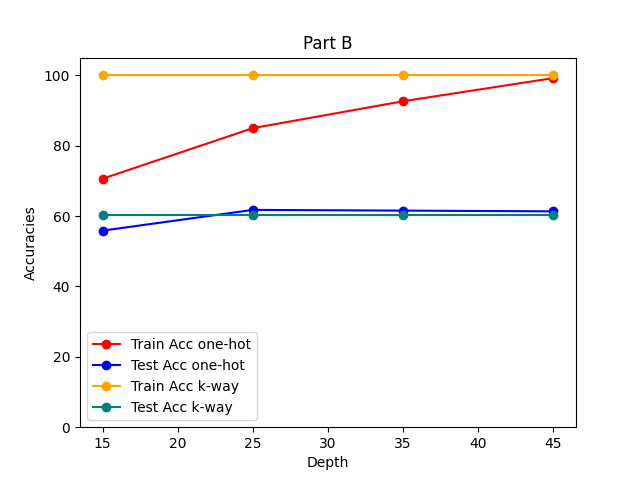
\includegraphics[width=0.9\textwidth]{./images/q1_part_b.png}
              \end{tabular}
          \end{center}




    \item The following Accuracy vs nodes graphs were obtained upon performing reduced error pruning for various depths

          \begin{center}
              \begin{center}
                  \begin{tabular}{c c}
                      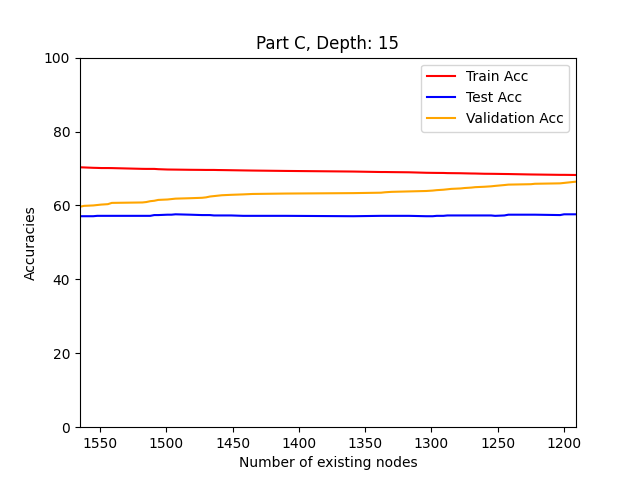
\includegraphics[width=0.40\textwidth]{./images/q1_part_c_depth15.png} & 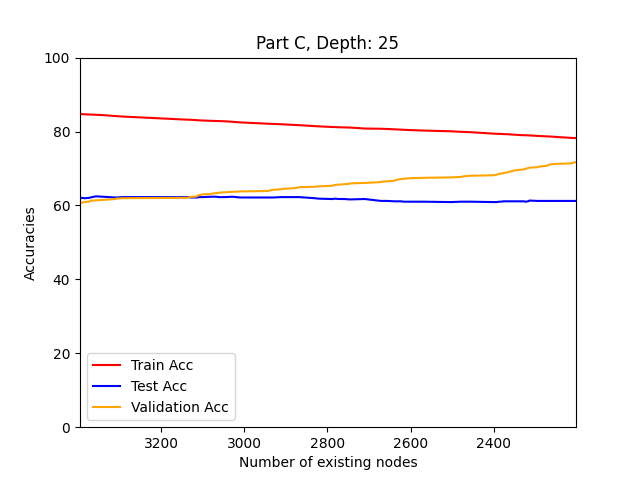
\includegraphics[width=0.40\textwidth]{./images/q1_part_c_depth25.png}
                  \end{tabular}
                  \begin{tabular}{c c}
                      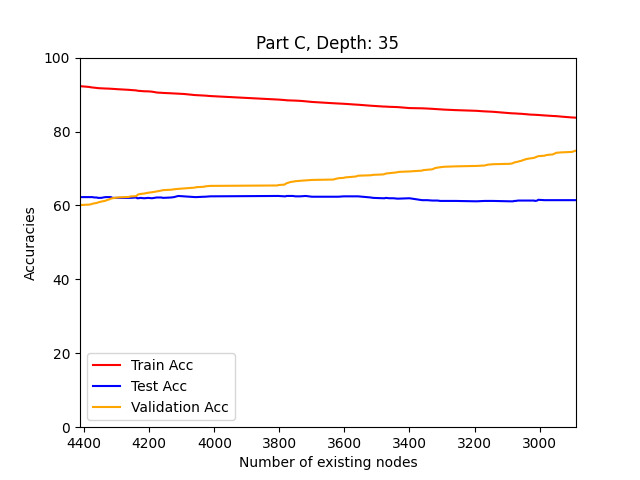
\includegraphics[width=0.40\textwidth]{./images/q1_part_c_depth35.png} & 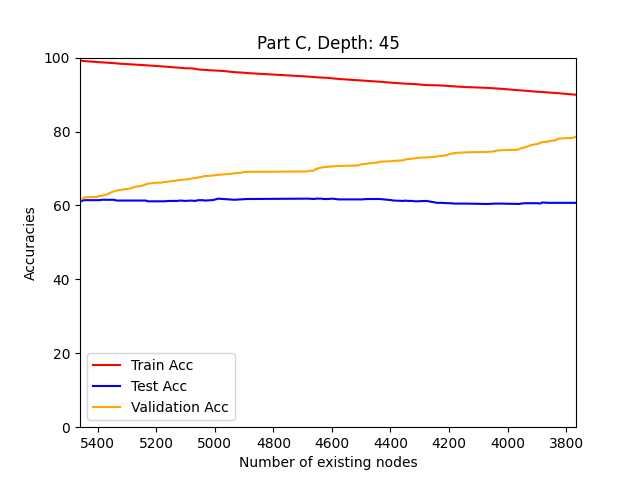
\includegraphics[width=0.40\textwidth]{./images/q1_part_c_depth45.png}
                  \end{tabular}
              \end{center}
          \end{center}

          Some observations to note:
          \begin{itemize}
              %   \item Pruning, with one-hot encoding:
              %         Time: 35.92s, Depth: 15, Train Acc: 68.24%, Test Acc: 57.60%, Val Acc: 66.44%
              %         Time: 108.66s, Depth: 25, Train Acc: 78.22%, Test Acc: 61.22%, Val Acc: 71.72%
              %         Time: 158.27s, Depth: 35, Train Acc: 83.74%, Test Acc: 61.43%, Val Acc: 74.83%
              %         Time: 210.50s, Depth: 45, Train Acc: 89.96%, Test Acc: 60.70%, Val Acc: 78.62%
              \item In all graphs the training accuracy decreases as number of nodes reduce in the graph (which suggests that more nodes could possibly lead to overfitting)
              \item Both the validation increases as number of nodes reduce in the graph
              \item we find that the test accuracies remain around the same value throughout the process
              \item In the initial stage of the DT (before pruning) we find the following order of accuracies:
                    \begin{itemize}
                        \item For depth 15: train $>$ val $>$ test accuracy
                        \item For all other depths: train $>$ test $>$ val accuracy
                    \end{itemize}
              \item As more nodes are pruned we find the following order of accuracies: train $>$ val $>$ test
          \end{itemize}


    \item Decision Tree using sci-kit learn

          \begin{enumerate}[label=\roman*.]
              \item Varying Max-Depth
                    \begin{itemize}
                        \item Training Set Accuracies:
                              \begin{itemize}
                                  % Updated
                                  \item Training Accuracy for max\_depth = 15 is 71.32
                                  \item Training Accuracy for max\_depth = 25 is 85.49
                                  \item Training Accuracy for max\_depth = 35 is 94.35
                                  \item Training Accuracy for max\_depth = 45 is 99.51
                              \end{itemize}
                        \item Test Set Accuracies:
                              \begin{itemize}
                                  \item Test Accuracy for max\_depth = 15 is 60.29
                                  \item Test Accuracy for max\_depth = 25 is 63.81
                                  \item Test Accuracy for max\_depth = 35 is 65.15
                                  \item Test Accuracy for max\_depth = 45 is 64.12
                              \end{itemize}
                        \item Validation Set Accuracies:
                              \begin{itemize}
                                  \item Validation Accuracy for max\_depth = 15 is 58.16
                                  \item Validation Accuracy for max\_depth = 25 is 61.61
                                  \item Validation Accuracy for max\_depth = 35 is 62.53
                                  \item Validation Accuracy for max\_depth = 45 is 61.95
                              \end{itemize}
                    \end{itemize}
                    \newpage
                    The obtained graph is as follows:
                    \begin{center}
                        \begin{tabular}{c}
                            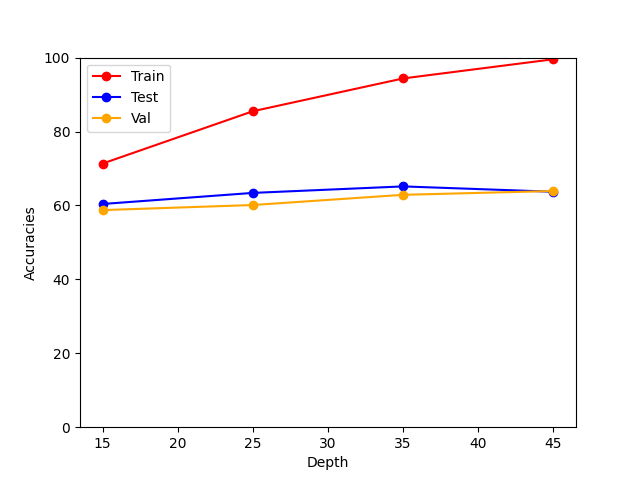
\includegraphics[width=0.8\textwidth]{./images/q1_part_d_depths.png}
                        \end{tabular}
                    \end{center}
                    We find that the best max\_depth obtained using the validation set is 35
              \item Varying ccp\_alpha
                    \begin{itemize}
                        \item Training Set Accuracies:
                              % Updated
                              \begin{itemize}
                                  \item Training Accuracy for ccp\_alpha = 0.001 is 68.94
                                  \item Training Accuracy for ccp\_alpha = 0.01 is 53.44
                                  \item Training Accuracy for ccp\_alpha = 0.1 is 50.33
                                  \item Training Accuracy for ccp\_alpha = 0.2 is 50.33
                              \end{itemize}
                        \item Test Set Accuracies:
                              \begin{itemize}
                                  \item Test Accuracy for ccp\_alpha = 0.001 is 66.29
                                  \item Test Accuracy for ccp\_alpha = 0.01 is 51.81
                                  \item Test Accuracy for ccp\_alpha = 0.1 is 49.64
                                  \item Test Accuracy for ccp\_alpha = 0.2 is 49.64
                              \end{itemize}
                        \item Validation Set Accuracies:
                              \begin{itemize}
                                  \item Validation Accuracy for max\_depth = 15 is 63.22
                                  \item Validation Accuracy for max\_depth = 25 is 50.00
                                  \item Validation Accuracy for max\_depth = 35 is 47.36
                                  \item Validation Accuracy for max\_depth = 45 is 47.36
                              \end{itemize}
                    \end{itemize}
                    \newpage
                    The obtained graph is as follows:
                    \begin{center}
                        \begin{tabular}{c}
                            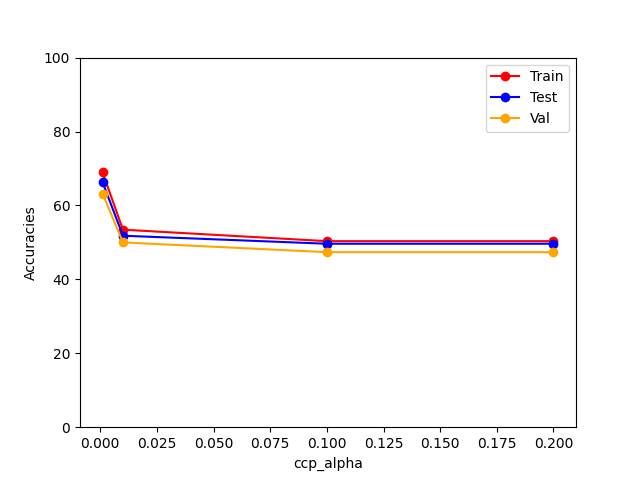
\includegraphics[width=0.8\textwidth]{./images/q1_part_d_pruning.png}
                        \end{tabular}
                    \end{center}
                    We find that the best ccp\_alpha obtained using the validation set is 0.001
              \item Observations to note:
                    \begin{itemize}
                        \item We find that the training data prediction accuracy is lesser in the sci-kit learn model compared to the model developed in both part b and c
                        \item On the other hand we find that the test data prediction accuracy is higher in the sci-kit model as compared to the model developed in both b and c
                    \end{itemize}
          \end{enumerate}

    \item Random Forests: Using out of box accuracies and grid search over the parameter space we observe the following result:
          \begin{itemize}
              \item Best Parameters:
                    \begin{itemize}
                        \item max\_features: 0.7
                        \item min\_samples\_split: 8
                        \item n\_estimators: 150
                    \end{itemize}
              \item Out of Box Accuracy: 71.8922
              \item Training Accuracy: 98.7990
              \item Test Accuracy: 71.7684
              \item Validation Accuracy: 69.5402
          \end{itemize}
          Compared to the previous parts, we find that the training, test and validation accuracy obtained here is higher than what was obtained in part d. However validation accuracy is lesser than what was obtained in part c (Training and Test accuracy are higher)



\end{enumerate}

\clearpage

\section{Neural Networks}

\begin{enumerate}[label=(\alph*)]
    \item A general Neural network architecture was created with configurable parameters such as:
          \begin{itemize}
              \item Mini-batch size: M
              \item Number of features: n
              \item Hidden layer architecture: [h1, h2, h3, ...]
              \item Target labels: r (number of target labels [1, 2, 3, ... r])
              \item Activation function: sigmoid, relu
              \item Learning rate, $\eta$: constant, adaptive
          \end{itemize}
          The terminating condition was fixed as 200 epochs. \\
          \emph{Incomplete}: I was able to make the structure in a way that it runs,
          but despite lot of efforts trying to debug,
          my accuracies weren't increasing and were changing around randomly between 10\% to 30\% for every epoch,
          and only predicting one class for all entries in a set of inputs for an epoch.

    \item Incomplete
          % part c
          %   \newpage
    \item Incomplete
          % part d
    \item  Incomplete
          % part e
    \item Incomplete
          % part f
    \item \underline{MLPClassifier} The following tables were obtained for various number of layers:
          \begin{enumerate}[label=\roman*.]
              \item 1 layer
                    \begin{table}[!htb]
                        \centering
                        \begin{tabular}{ccccc}
                            \hline
                            Class & Precision & Recall & F1Score & Support \\ \hline
                            1.0   & 0.70      & 0.91   & 0.79    & 1971    \\
                            2.0   & 0.52      & 0.44   & 0.48    & 1978    \\
                            3.0   & 0.47      & 0.34   & 0.40    & 1952    \\
                            4.0   & 0.44      & 0.33   & 0.38    & 2008    \\
                            5.0   & 0.58      & 0.79   & 0.67    & 2091    \\ \hline
                        \end{tabular}
                        \caption{train}
                        \label{part f train depth 1}
                    \end{table}
                    \begin{table}[!htb]
                        \centering
                        \begin{tabular}{ccccc}
                            \hline
                            Class & Precision & Recall & F1Score & Support \\ \hline
                            1     & 0.91      & 0.90   & 0.74    & 230     \\
                            2     & 0.67      & 0.70   & 0.69    & 190     \\
                            3     & 0.55      & 0.58   & 0.57    & 190     \\
                            4     & 0.57      & 0.49   & 0.53    & 218     \\
                            5     & 0.66      & 0.72   & 0.69    & 172     \\ \hline
                        \end{tabular}
                        \caption{test}
                        \label{part f test depth 1}
                    \end{table}
                    \newpage
              \item 2 layers
                    \begin{table}[!htb]
                        \centering
                        \begin{tabular}{ccccc}
                            \hline
                            Class & Precision & Recall & F1Score & Support \\ \hline
                            1.0   & 0.76      & 0.90   & 0.83    & 1971    \\
                            2.0   & 0.58      & 0.53   & 0.55    & 1978    \\
                            3.0   & 0.46      & 0.41   & 0.43    & 1952    \\
                            4.0   & 0.46      & 0.36   & 0.40    & 2008    \\
                            5.0   & 0.63      & 0.78   & 0.70    & 2091    \\ \hline
                        \end{tabular}
                        \caption{train}
                        \label{part f train depth 2}
                    \end{table}
                    \begin{table}[!htb]
                        \centering
                        \begin{tabular}{ccccc}
                            \hline
                            Class & Precision & Recall & F1Score & Support \\ \hline
                            1     & 0.93      & 0.90   & 0.71    & 236     \\
                            2     & 0.71      & 0.68   & 0.70    & 206     \\
                            3     & 0.52      & 0.58   & 0.55    & 178     \\
                            4     & 0.56      & 0.49   & 0.52    & 211     \\
                            5     & 0.65      & 0.72   & 0.68    & 169     \\ \hline
                        \end{tabular}
                        \caption{test}
                        \label{part f test depth 2}
                    \end{table}
                    % \newpage
              \item 3 layers
                    \begin{table}[!htb]
                        \centering
                        \begin{tabular}{ccccc}
                            \hline
                            Class & Precision & Recall & F1Score & Support \\ \hline
                            1.0   & 0.80      & 0.89   & 0.84    & 1971    \\
                            2.0   & 0.61      & 0.58   & 0.59    & 1978    \\
                            3.0   & 0.50      & 0.44   & 0.47    & 1952    \\
                            4.0   & 0.46      & 0.42   & 0.44    & 2008    \\
                            5.0   & 0.65      & 0.74   & 0.69    & 2091    \\ \hline
                        \end{tabular}
                        \caption{train}
                        \label{part f train depth 3}
                    \end{table}
                    \begin{table}[!htb]
                        \centering
                        \begin{tabular}{ccccc}
                            \hline
                            Class & Precision & Recall & F1Score & Support \\ \hline
                            1     & 0.90      & 0.92   & 0.91    & 223     \\
                            2     & 0.70      & 0.71   & 0.70    & 197     \\
                            3     & 0.54      & 0.61   & 0.57    & 175     \\
                            4     & 0.47      & 0.50   & 0.48    & 176     \\
                            5     & 0.80      & 0.66   & 0.72    & 229     \\ \hline
                        \end{tabular}
                        \caption{test}
                        \label{part f test depth 3}
                    \end{table}
              \item 4 layers
                    \begin{table}[!htb]
                        \centering
                        \begin{tabular}{ccccc}
                            \hline
                            Class & Precision & Recall & F1Score & Support \\ \hline
                            1.0   & 0.82      & 0.88   & 0.85    & 1971    \\
                            2.0   & 0.62      & 0.62   & 0.62    & 1978    \\
                            3.0   & 0.50      & 0.45   & 0.47    & 1952    \\
                            4.0   & 0.46      & 0.43   & 0.45    & 2008    \\
                            5.0   & 0.66      & 0.73   & 0.69    & 2091    \\ \hline
                        \end{tabular}
                        \caption{train}
                        \label{part f train depth 4}
                    \end{table}
                    \begin{table}[!htb]
                        \centering
                        \begin{tabular}{ccccc}
                            \hline
                            Class & Precision & Recall & F1Score & Support \\ \hline
                            1     & 0.86      & 0.93   & 0.90    & 212     \\
                            2     & 0.66      & 0.70   & 0.68    & 187     \\
                            3     & 0.51      & 0.59   & 0.55    & 174     \\
                            4     & 0.51      & 0.49   & 0.50    & 195     \\
                            5     & 0.81      & 0.66   & 0.73    & 232     \\ \hline
                        \end{tabular}
                        \caption{test}
                        \label{part f test depth 4}
                    \end{table}
                    \newpage


          \end{enumerate}
          We obtain the following graph:
          \begin{center}
              \begin{tabular}{c}
                  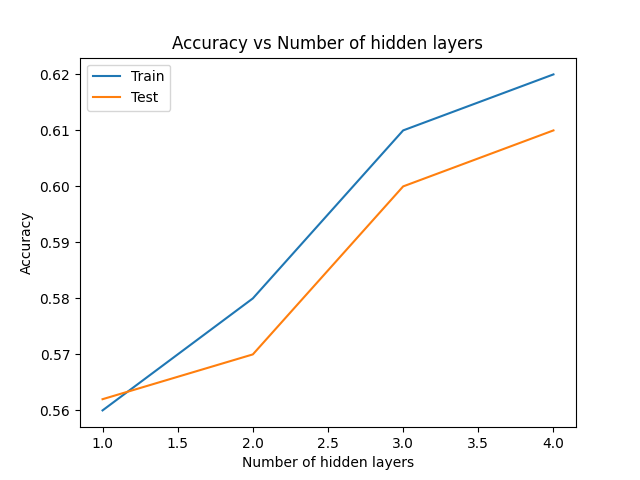
\includegraphics[width=0.9\textwidth]{./images/part_f.png}
              \end{tabular}
          \end{center}

\end{enumerate}

\end{document}
